\documentclass[a4paper]{article}
\usepackage[letterpaper,margin=1in]{geometry}
\usepackage{blindtext}
\usepackage{lastpage}
\usepackage{fancyhdr}
\usepackage{setspace}
\usepackage{amsmath}
\usepackage{graphicx}
\usepackage{float}
\usepackage{matlab-prettifier}
\usepackage{hyperref}
\usepackage{titlesec}


\graphicspath{{./Figures}}

\pagestyle{fancy} % Enable fancy headers
\fancyhead[L]{CE 591} % Left-aligned header
\fancyhead[C]{Wave Hydrodynamics} % Centered header
\fancyhead[R]{10/04/2025} % Right-aligned header

\onehalfspacing

\begin{document}

\titleformat{\section}
  {\normalfont\bfseries\fontsize{12}{10}\selectfont}
  {\large\thesection.} 
  {0.5em}
  {}

\thispagestyle{empty}

\begin{figure}[H]
    \vspace{1.2cm}
    \centering
    
\includegraphics[width=0.5\textwidth]{logo.png}
\end{figure}
\vspace{1cm}

\begin{center}
    \textbf{\LARGE Middle East Technical University}
    \vspace{0.3cm}

    \textbf{\LARGE Department of Civil Engineering}
    \vspace{0.5cm}

    \textbf{\Large 2024-2025 Spring Semester}
    \vspace{1.5cm}

    \textbf{\Large CE 591 Wave Hydrodynamics}
    \vspace{0.3cm}

    \textbf{\Large Homework 1}
    \vspace{2.8cm}

    \textbf{\large Student Name: }\large Bilge Kutay
    
    \textbf{\large Student ID: }\large 2511798
    \vspace{0.8cm}

    \textbf{\large Date: }\large 10/04/2025
\end{center}

\newpage
\tableofcontents
\newpage

\section{Question 1} Select a coastal engineering problem (in regional scale), and discuss which
governing equations can be used to model the waves for your selected problem. Explain the reason
why you have selected these equations with a few paragraphs.
\vspace{0.3cm}

A key problem in coastal engineering involves modeling non-linear wave transformation as waves propagate from deep to shallow water. This process includes shoaling, refraction, and breaking, which are governed by the Boussinesq equations and the Korteweg-de Vries (KdV) equation. These equations are selected for their ability to balance nonlinear and dispersive effects, critical for simulating wave behavior in shallow coastal zones.

The Boussinesq equations simplify the Navier-Stokes equations by retaining nonlinear and dispersive terms while reducing complexity. Unlike linear wave theory, which assumes small wave amplitudes and ignores non-linear interactions, the Boussinesq captures wave steepening, energy transfer, and frequency dispersion. This makes it effective for predicting wave asymmetry and breaking in shallow water.

The KdV equation supports this approach by focusing on weakly non-linear and weakly dispersive waves, such as solitary waves or long waves in shallow water. It provides a simplified model for unidirectional wave propagation, ideal for scenarios like tsunami evolution or wave deformation over gentle slopes. While higher-order Stokes theories are accurate for deep-water waves, they become impractical in shallow environments due to their reliance on perturbation methods.

In summary, the Boussinesq and KdV equations provide a practical mathematical foundation for modeling wave transformation, addressing the limitations of linear theory and higher-order Stokes models. 

\vspace{0.5cm}
\section{Question 2} Considering Stokes’ second-order wave theory for monochromatic waves, do the following computations and compare your results with the solutions from linear theory. Take wave height H = 3 m, wave period T = 8 s and water depth h = 25 m.
\vspace{0.3cm}

\noindent\textbf{(a)} Plot the surface elevation for at least one wave period.
\vspace{0.2cm}

The plot in Figure 1 shows the surface elevation of a Stokes' second-order wave at x = 0 and t = 0-8. The surface elevation is calculated using the following equations:

\[\eta_1 = \frac{H}{2} \cos(\theta)\]
\[\eta_2 = \frac{1}{16} k H^2 \left(3 \coth^3(kh) - \coth(kh)\right) \cos(2\theta)\]
\[\eta = \eta_1 + \eta_2\]

\begin{figure}[H]
    \centering
    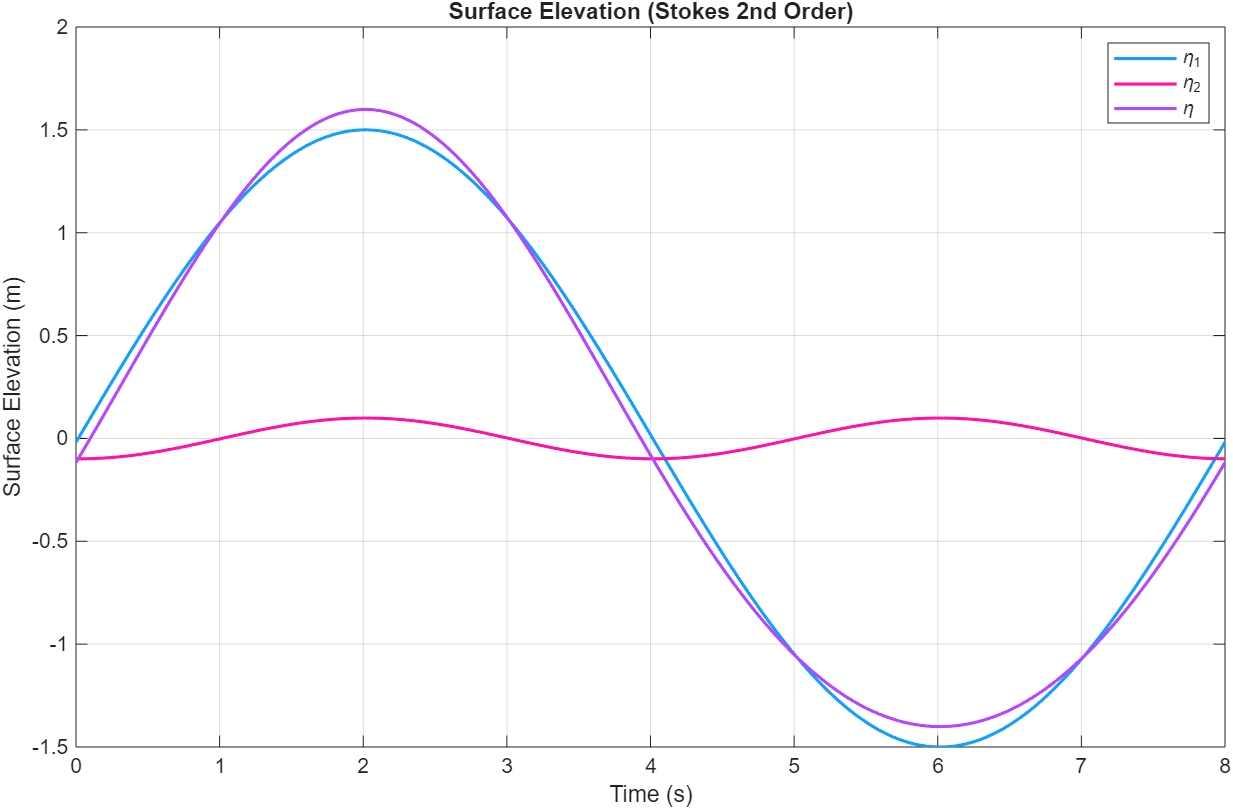
\includegraphics[width=0.8\textwidth]{CE591HW1-Q1a.png}
    \caption{\small Surface elevation plot for Stokes' second-order wave theory.}
    \label{fig:plot2a}
\end{figure}
\vspace{0.3cm}

The surface elevation plot illustrates Stokes’ second-order wave theory, combining a first-order sinusoidal wave ($\eta_1$) and a smaller second-order correction ($\eta_2$). The linear term ($\eta_1$) dominates the wave shape, while $\eta_2$ introduces asymmetry by sharpening crests and flattening troughs. At crests, $\eta_2$ adds to $\eta_1$, increasing peak height. At troughs, $\eta_2$ opposes $\eta_1$, reducing depth. The second-order term remains minor caused by the weak non-linearity. This confirms Stokes’ theory accurately models wave steepening under the given conditions.
\vspace{0.3cm}

\noindent\textbf{(b)} Make a plot of the vertical variation of horizontal (\(u\)) and vertical (\(w\)) particle velocities
\vspace{0.2cm}

Figures 2 and 3 show the vertical variation of horizontal (\(u\)) and vertical (\(w\)) particle velocities at \(t = 4\) and \(x = 0\) for Stokes' second-order wave theory. The velocities are calculated using the following equations:

\[u_1 = \frac{H \omega}{2} \cdot \frac{\cosh(k(h+z))}{\sinh(kh)} \cos(\omega t - kx)\]
\[u_2 = \frac{3}{16} c (kH)^2 \cdot \frac{\cosh(2k(z+h))}{\sinh^4(kh)} \cos(2\theta)\]
\[u = u_1 + u_2\]

\[w_1 = -\frac{H \omega}{2} \cdot \frac{\sinh(k(h+z))}{\sinh(kh)} \sin(\omega t - kx)\]
\[w_2 = -\frac{3}{16} \cdot \frac{\sinh(2k(z+h))}{\sinh^4(kh)} \sin(2\theta)\]
\[w = w_1 + w_2\]

\begin{figure}[H]
    \centering
    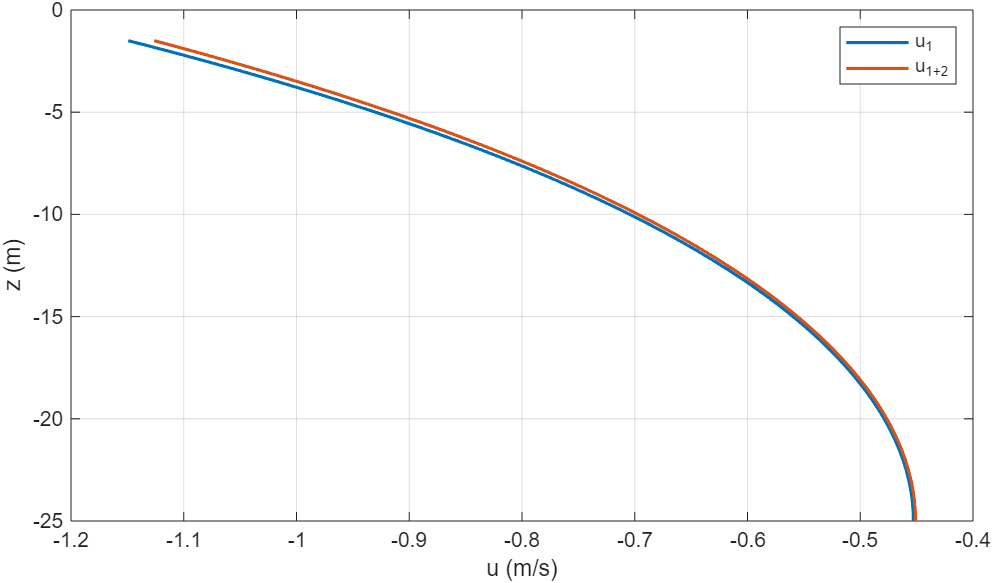
\includegraphics[width=0.8\textwidth]{CE591HW1-Q1b.png}
    \caption{\small Horizontal velocity profiles for Stokes' second-order wave theory.}
    \label{fig:plot2b}
\end{figure}


\begin{figure}[H]
    \centering
    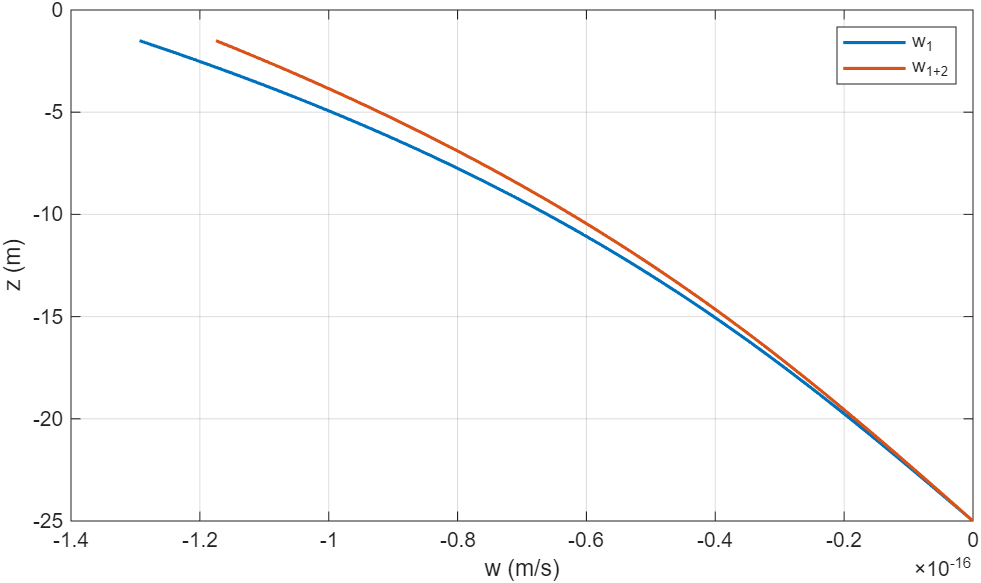
\includegraphics[width=0.8\textwidth]{CE591HW1-Q1b_2.png}
    \caption{\small Vertical velocity profiles for Stokes' second-order wave theory.}
    \label{fig:plot2.2b}
\end{figure}
\vspace{0.3cm}

The velocity profiles illustrate the variation of horizontal (\(u\)) and vertical (\(w\)) particle velocities with depth. At \(t = 4\) and \(x = 0\), the particles are positioned at the wave trough, where both \(u\) and \(w\) attain their maximum negative values, signifying motion in the direction opposite to wave propagation. The velocities exhibit a gradual reduction with depth, with \(u\) decreasing at a slower rate compared to \(w\). This behavior aligns with Stokes' second-order wave theory, which accounts for the contributions of both linear and non-linear terms to \(u\), while \(w\) mainly reflects the oscillatory nature of the wave motion. Near the seabed, \(w\) approaches zero, while \(u\) remains non-zero, indicating the continued presence of horizontal motion even near the seabed.
\vspace{0.3cm}

\noindent\textbf{(c)} Repeat the calculations in Part (b), changing the water depth as \( h = 20 \, \text{m} \) and \( h = 30 \, \text{m} \). Compare your results with your results from Part (b).
\vspace{0.3cm}

Changing the water depth to \( h = 20 \, \text{m} \) and \( h = 30 \, \text{m} \) alters the velocity profiles:  

\begin{itemize}  
    \item {Shallower depth (\( h = 20 \, \text{m} \))}: Increased bottom influence causes the horizontal velocity to intensify near the surface due to energy concentration, while vertical velocity exhibits more rapid decrease with depth as bottom boundary effects become more dominant. 
    \begin{figure}[H]
        \centering
        \begin{minipage}{0.49\textwidth}
            \centering
            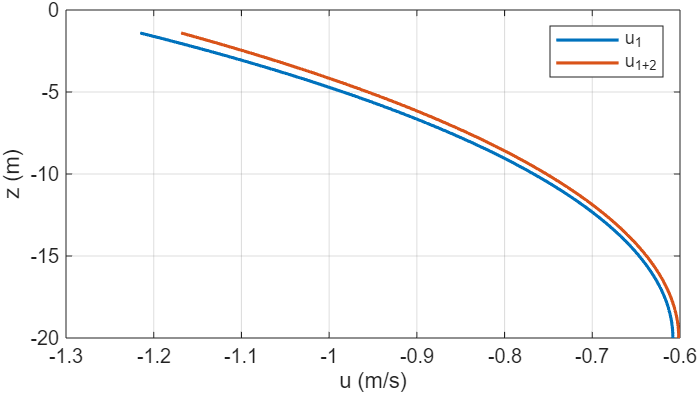
\includegraphics[width=\textwidth]{CE591HW1-Q1c1.png}
            \caption{\small Horizontal velocity profiles for h = 20 m.}
            \label{fig:plot2c_1}
        \end{minipage}
        \hfill
        \begin{minipage}{0.49\textwidth}
            \centering
            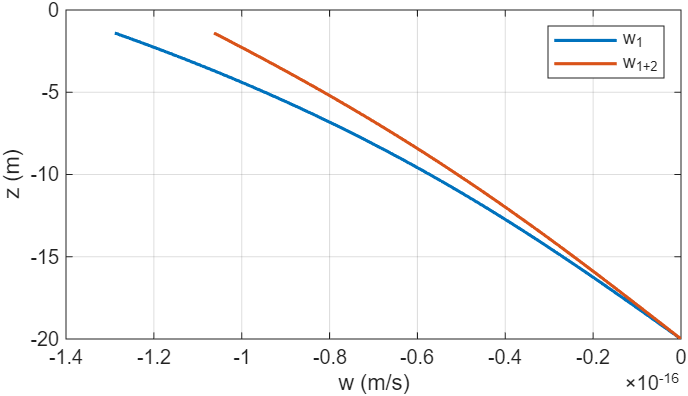
\includegraphics[width=\textwidth]{CE591HW1-Q1c2.png}
            \caption{\small Vertical velocity profiles for h = 20 m.}
            \label{fig:plot2c_2}
        \end{minipage}
    \end{figure}

    \item {Deeper depth (\( h = 30 \, \text{m} \))}: Bottom inffluence decreases with increased depth. The horizontal velocity weakens near the surface, while the vertical velocity decays more gradually with depth. 
    \begin{figure}[H]
        \centering
        \begin{minipage}{0.49\textwidth}
            \centering
            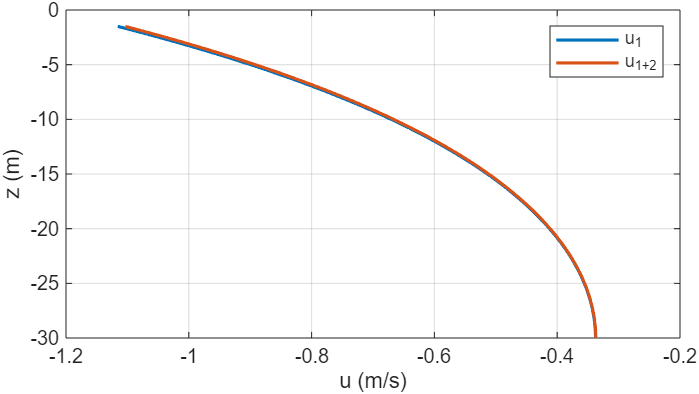
\includegraphics[width=\textwidth]{CE591HW1-Q1c3.png}
            \caption{\small Horizontal velocity profiles for h = 30 m.}
            \label{fig:plot2c_3}
        \end{minipage}
        \hfill
        \begin{minipage}{0.49\textwidth}
            \centering
            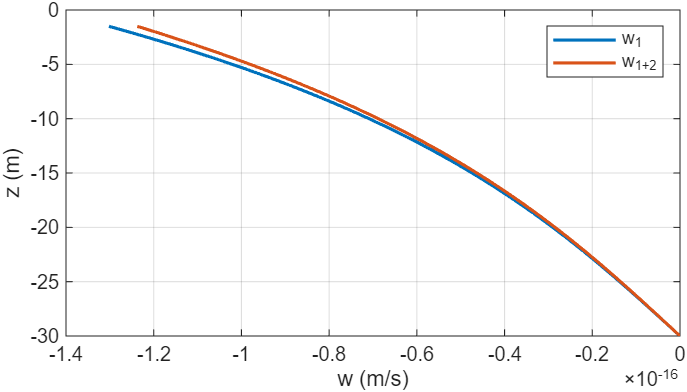
\includegraphics[width=\textwidth]{CE591HW1-Q1c4.png}
            \caption{\small Vertical velocity profiles for h = 30 m.}
            \label{fig:plot2c_4}
        \end{minipage}
    \end{figure}

\end{itemize}  
\vspace{0.5cm}

\noindent\textbf{(d)} Non-dimensional dynamic pressure can be calculated by dividing the dynamic pressure with $\rho$g$\eta$. Plot the vertical variation of the non-dimensional dynamic pressure as a function of z/h at \( h = 20 \, \text{m} \), \( h = 25 \, \text{m} \) and \( h = 30 \, \text{m} \).
\vspace{0.3cm}

Figure 8 shows the dynamic pressure profiles for different water depths. The dynamic pressure is calculated using the following equation:

\[
P_d = \frac{\cosh(k(z+h))}{\cosh(kh)}
\]

\begin{figure}[H]
    \centering
    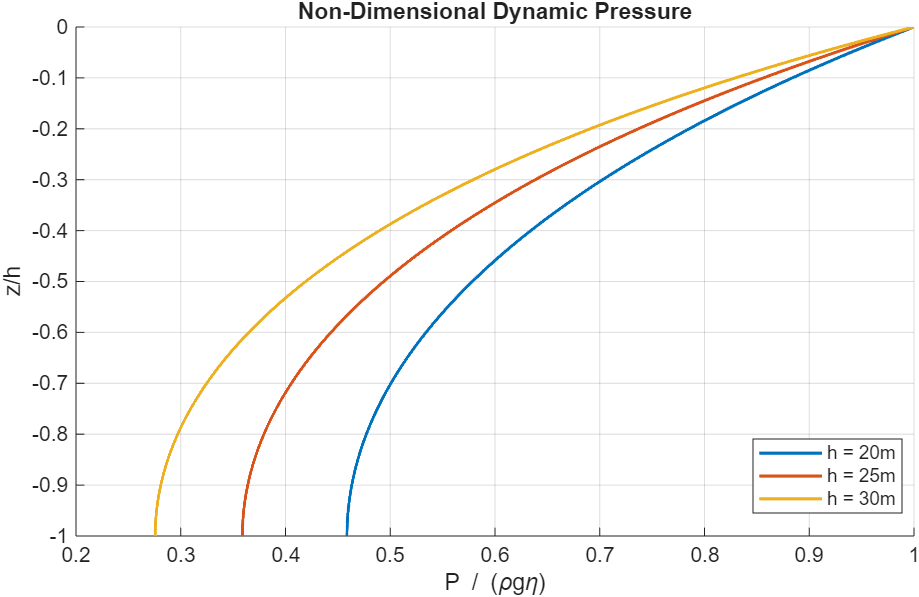
\includegraphics[width=0.8\textwidth]{CE591HW1-Q1d.png}
    \caption{\small Dynamic pressure profiles for different water depths.}
    \label{fig:plot2d}
\end{figure} 

\section{Question 3} Write a program that calculates the water surface elevation of a solitary wave for a given solitary wave height H and water depth h. Plot the water surface elevation for H = 0.074 m and h = 30 cm. Compare your theoretical calculation and experimental measurements. Discuss potential discrepancies.
\vspace{0.3cm}

\begin{figure}[H]
    \centering
    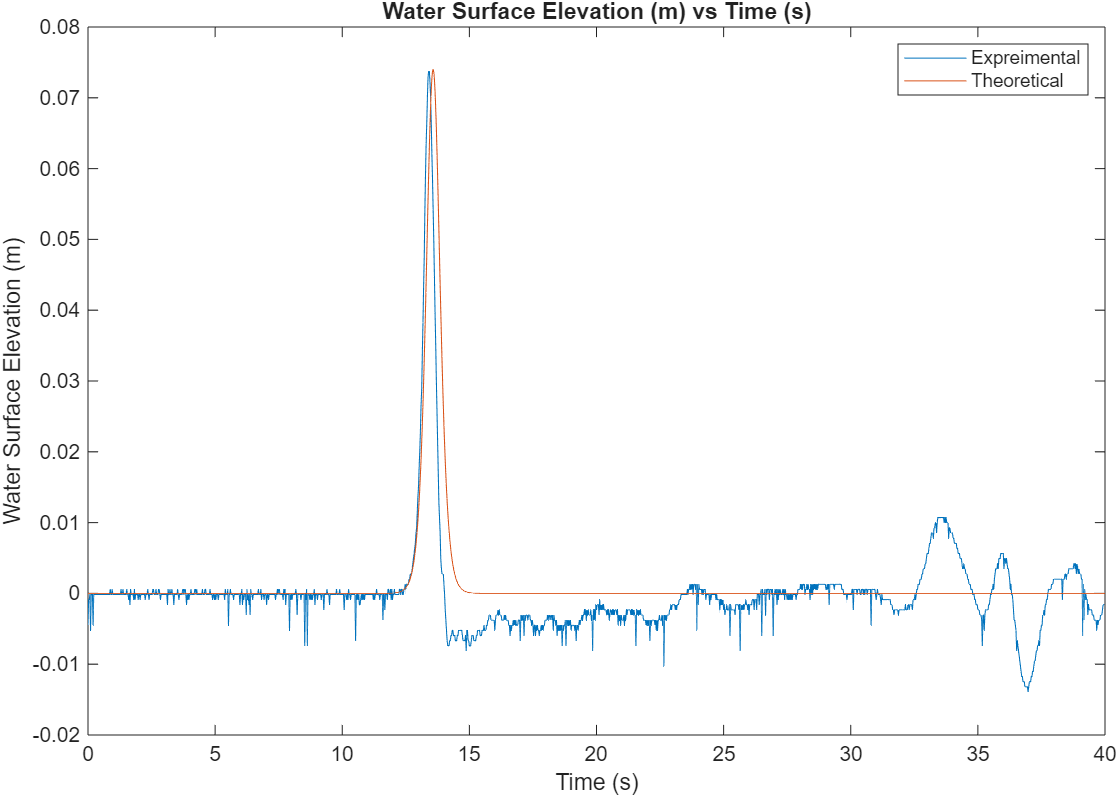
\includegraphics[width=0.67\textwidth]{CE591HW1-Q3.png}
    \caption{\small Surface elevation of a solitary wave.}
    \label{fig:plot3}
\end{figure} 

The surface elecation of the solitary wave is calculated using the following equations:

\[X = x - c \cdot t\] 
\[c = \sqrt{g \cdot (h+H)}\]. 
\[\eta = H \cdot \text{sech}^2\left(X \cdot \sqrt{\frac{3H}{4h^3}}\right)\]

The comparison between theoretical and experimental solitary wave profiles shows a good match, with some expected discrepancies. The theoretical model assumes ideal conditions, while experimental data may be influenced by factors like wave reflection, bottom friction, and measurement errors. The experimental data also shows some oscillations, likely caused by wave interactions or reflections. Overall, the theoretical model provides a solid foundation for solitary waves, but real-world conditions can introduce variations that need to be considered in practical applications.
\vspace{0.5cm}

\section{Question 4} Write a program utilizing cnoidal wave theory summarized in your lecture notes for a given wave height H, wave period T and water depth h. Plot the water surface elevations for at least three selected waves on the same figure for two wave periods. Describe the procedure you have used and discuss your results.

\subsection*{Procedure}
The MATLAB program calculates the water surface elevation of cnoidal waves using the following steps:

\begin{enumerate}
    \item \textbf{Selection of Wave Parameters:}
    \begin{itemize}
        \item The wave height \(H\), wave period \(T\), and water depth \(h\) were chosen to be within the applicable range for cnoidal waves. This ensures that the assumptions of cnoidal wave theory are valid and the results are physically meaningful.
    \end{itemize}

    \begin{figure}[H]
        \centering
        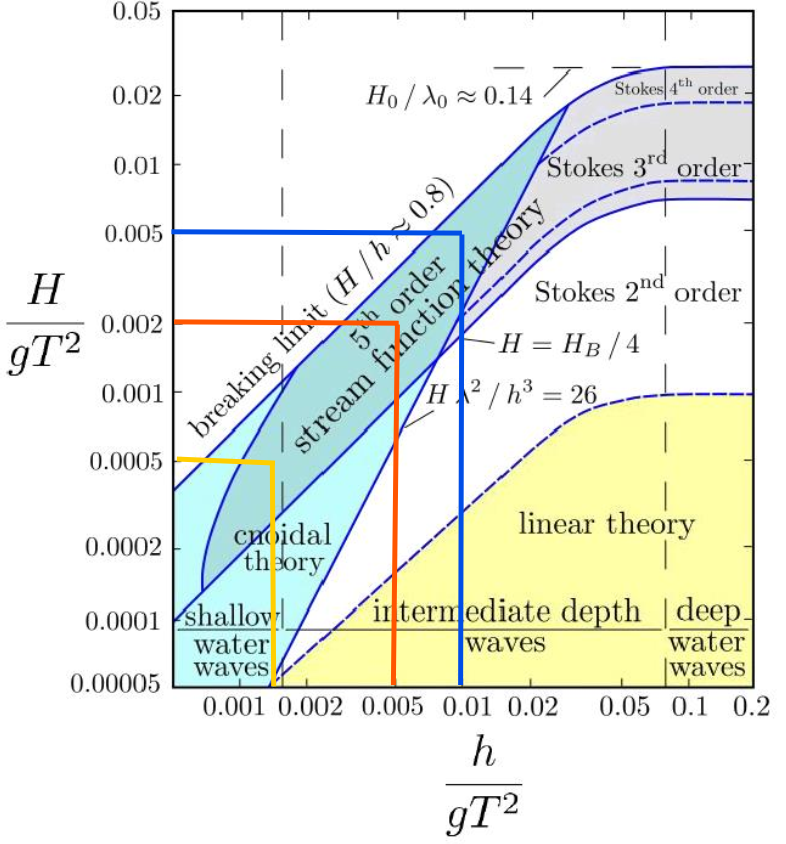
\includegraphics[width=0.38\textwidth]{CE591HW1-Q4.1.png}
        \caption{\small Ranges of applicability for various wave theories.}
        \label{fig:wavetheory}
    \end{figure}

    \item \textbf{Initialization of Parameters:}
    \begin{itemize}
        \item The program begins by defining constants such as gravitational acceleration (\(g = 9.81 \, \text{m/s}^2\)) and coefficients (\(a_0, b_0, a_1, b_1, a_2, b_2, e_1, f_1, e_2, f_2\)) that are used in the cnoidal wave theory. These coefficients are derived from approximations of elliptic integrals and are essential for accurately modeling the wave properties.
    \end{itemize}

    \item \textbf{Outer Loop for Ursell Number (\(Ur\)) and Parameter \(A\):}
    \begin{itemize}
        \item The outer loop iteratively calculates the Ursell number (\(Ur\)) and the parameter \(A\), which represents the wave nonlinearity. These values are updated until the error is less than the tolerance or the maximum number of iterations is reached.
        \item The wavelength (\(L_c\)) is calculated using the formula:
        \[
        L_c = T \cdot \sqrt{\frac{g}{h}} \cdot \sqrt{1 + \frac{H}{h} \cdot A} \cdot h
        \]
        \item The Ursell number (\(Ur\)) is then calculated as:
        \[
        Ur = H \cdot \frac{L_c^2}{h^3}
        \]
    \end{itemize}

    \item \textbf{Inner Loop for Parameter \(m_1\):}
    \begin{itemize}
        \item The inner loop uses the Newton-Raphson method to iteratively calculate the parameter \(m_1\), which is related to the elliptic parameter (\(m\)) of the cnoidal wave.
        
        \item The elliptic integral approximation (\(K\)) and its derivative (\(dK\)) are calculated using:
        \[
        K = a_0 + a_1 m_1 + a_2 m_1^2 - (b_0 + b_1 m_1 + b_2 m_1^2) \ln(m_1)
        \]
        \[
        dK = a_1 + 2 a_2 m_1 + (b_1 + 2 b_2 m_1) \ln(m_1) - \frac{b_0 + b_1 m_1 + b_2 m_1^2}{m_1}
        \]

        \item The function \(f(m_1)\) and its derivative \(f'(m_1)\) are defined as:
        \[
        f(m_1) = 1 - m_1 - \frac{3}{16} \cdot \frac{Ur}{K^2}
        \]
        \[
        f'(m_1) = \frac{3}{8} \cdot \frac{Ur}{K^3} \cdot dK - 1
        \]
        
        \item The parameter \(m_1\) is updated using the Newton-Raphson formula:
        \[
        m_1^{\text{new}} = m_1 - \frac{f(m_1)}{f'(m_1)}
        \]
        The error is calculated as the absolute difference between the new and old values of \(m_1\), and the loop continues until the error is less than the tolerance.
    \end{itemize}
    \vspace{1.5cm}

    \item \textbf{Calculation of \(m\) and Update of \(A\):}
    \begin{itemize}
        \item After the inner loop converges, the elliptic modulus (\(m\)) is calculated as:
        \[
        m = 1 - m_1
        \]
        \item The complete elliptic integral approximation (\(E\)) is calculated using:
        \[
        E = (1 + e_1 m_1 + e_2 m_1^2) - (f_1 m_1 + f_2 m_1^2) \ln(m_1)
        \]
        \item The parameter \(A\) is updated using:
        \[
        A^{\text{new}} = \frac{2}{m} - 1 - \frac{3}{m} \cdot \frac{E}{K}
        \]
        The error is calculated as the absolute difference between the new and old values of \(A\), and the outer loop continues until the error is less than the tolerance.
    \end{itemize}

    \item \textbf{Calculation of Wave Properties:}
    \begin{itemize}
        \item After the outer loop converges, the following wave properties are calculated:
        \begin{itemize}
            \item \textbf{Wave number (\(K_c\))}:
            \[
            K_c = \frac{2 \cdot K(m)}{L_c}
            \]
            \item \textbf{Wave celerity (\(c_c\))}:
            \[
            c_c = \sqrt{g \cdot (h + A \cdot H)}
            \]
            \item \textbf{Parameter \(B\)}:
            \[
            B = \frac{1}{m} \left(1 - m - \frac{E(m)}{K(m)}\right)
            \]
        \end{itemize}
    \end{itemize}

    \item \textbf{Calculation and Plotting of Surface Elevation:}
    \begin{itemize}
        \item The spatial (\(x\)) and temporal (\(t\)) domains are defined.
        \item The surface elevation (\(\eta\)) is calculated using the cnoidal wave formula:
        \[
        \eta = H \cdot \left(B + \text{cn}^2\left(K_c \cdot (x - c_c \cdot t), m\right)\right)
        \]
        \item The surface elevation is plotted over time, showing the periodic nature of the cnoidal wave and its dependence on the wave parameters.
    \end{itemize}
\end{enumerate}

\begin{figure}[H]
    \centering
    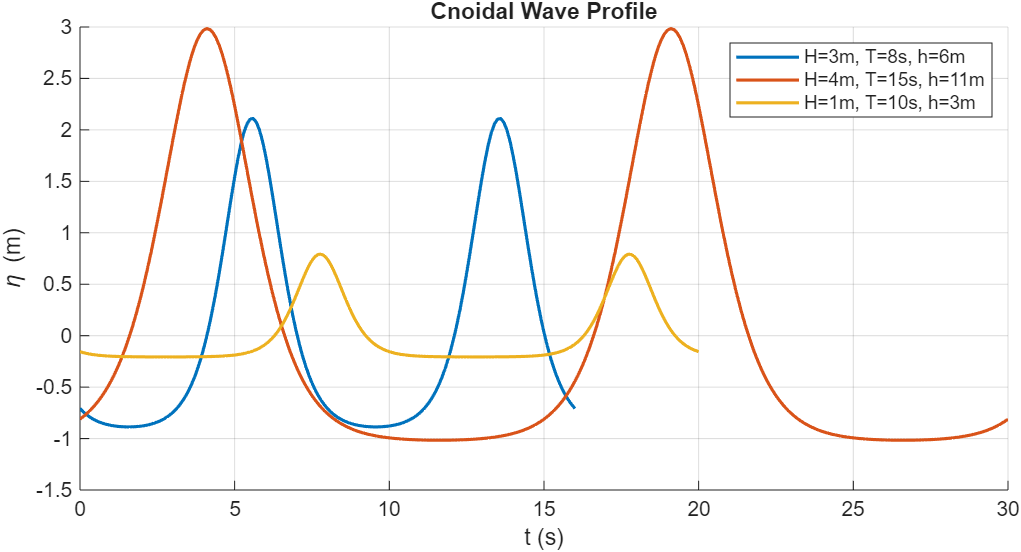
\includegraphics[width=0.8\textwidth]{CE591HW1-Q4.png}
    \caption{\small Cnoidal wave surface elevation.}
    \label{fig:plot4}
\end{figure} 

\section{Question 5} In this question, you will generate a computational mesh using blockMesh utility of OpenFOAM. A wave will be generated using first-order wave theory in this flume. Generate a 2D computational mesh based on the information given.


The mesh is generated with 1 m length in z direction, 25 m length in x direction and 0.1 m height in y direction. At x = 8.5 m, the slope of 1:25 is taken into account for the seabed. Using these coordinates, the vertices of the block is formed in the blockMeshDict file. It is then divided into 850 and 1650 cells in x direction for two blocks, 1 cell in y direction and 280 cells in z direction. To obtain the cell count for the z direction, the first cell size of $7.5 \cdot 10^{-4}$ m and last cell size of 0.01 m are used. The last cell size is selected to keep the aspect ratio equal to 1 at the free-surface. The grading on the z-direction is calculated to be 13.333 based on the first and last cell sizes and the total length.

\begin{figure}[H]
    \centering
    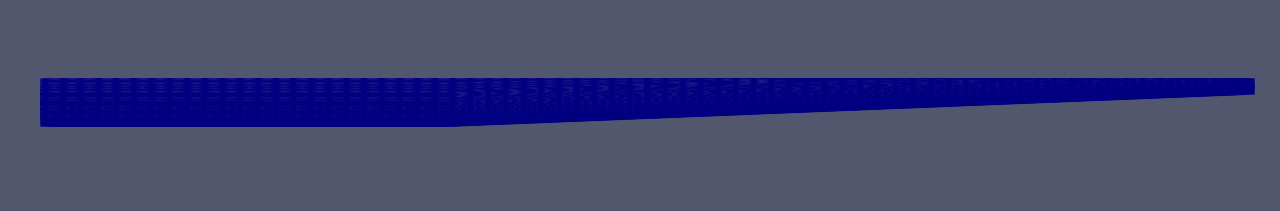
\includegraphics[width=1\textwidth]{mesh1.png}
    \caption{\small 2D computational mesh generated using blockMesh utility of OpenFOAM.}
    \label{fig:mesh1}
\end{figure} 
\vspace{0.3cm}
\begin{figure}[H]
    \centering
    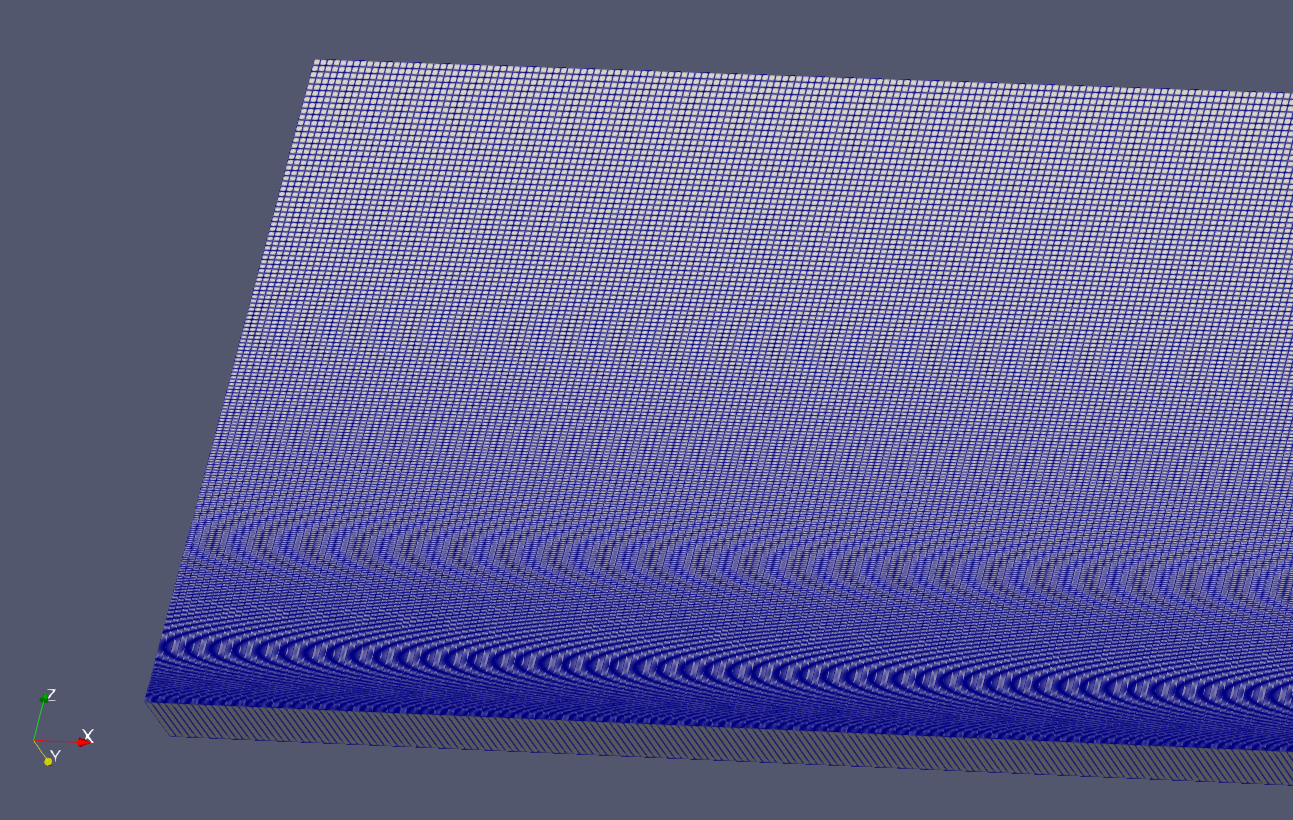
\includegraphics[width=0.6\textwidth]{mesh2.png}
    \caption{\small Inlet part of the mesh.}
    \label{fig:mesh2}
\end{figure} 
\vspace{0.3cm}
\begin{figure}[H]
    \centering
    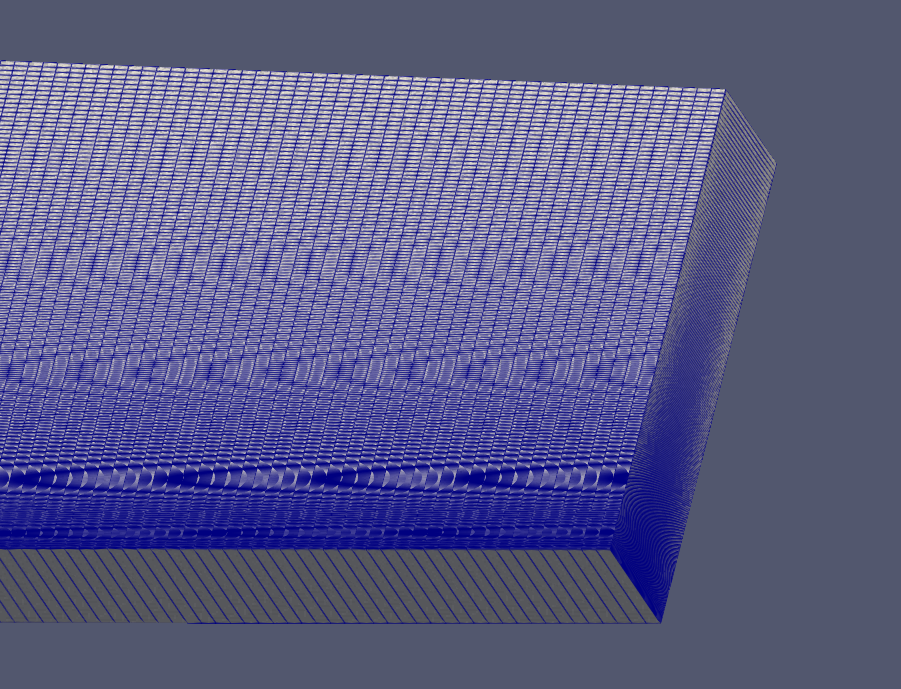
\includegraphics[width=0.6\textwidth]{mesh3.png}
    \caption{\small Outlet part of the mesh.}
    \label{fig:mesh3}
\end{figure} 
\vspace{0.3cm}

The total number of cells in the mesh is \textbf{700,000}, the minimum cell area is \textbf{$2.547 \cdot 10^{-6}$ m}, the maximum cell area is \textbf{0.001 m}, and the maximum aspect ratio is \textbf{1}, as obtained from the checkMesh function.

\newpage

\begin{thebibliography}{99}
    \bibitem{CE591} CE591 Lecture Notes. (2025). 
    \bibitem{CoastalBook} Ergin, A. (2019). \textit{Coastal engineering} (2nd ed.). Middle East Technical University Development Foundation Publishing and Communications Co.
    \bibitem{GitHubCopilot} Microsoft. (2021). \textit{GitHub Copilot} [Large language model]. GitHub. Retrieved from \url{https://github.com/features/copilot}
\end{thebibliography}

\newpage
\appendix

\section{Appendix}

\section*{\small MATLAB function for Stokes' second-order wave theory surface elevation}
\begin{lstlisting}[frame=single, numbers=left, style=Matlab-Pyglike]
function stokes_surface_profile(T, h)
    H = 3;
    L = 1.56*T^2; 
    tol = 3e-5;
    err = tol + 1;

    while err > tol
        L_new = 9.81*(T^2) * tanh(2*pi*h/L) / (2*pi);
        err = abs(L-L_new);
        L= L_new;
    end

    k = 2*pi/L;
    omega = 2*pi/T;
    t = 0:0.01:T;
    x = 0;
    theta = omega*t - k*x;

    eta_1 = (H/2) * cos(theta);
    eta_2 = (1/16) * k * H^2 * (3*coth(k*h)^3 - coth(k*h)) .* cos(2*theta);
    eta = eta_1 + eta_2;

    plot(t, eta_1, 'LineWidth', 1.5)
    hold on
    plot(t, eta_2, 'LineWidth', 1.5)
    hold on
    plot(t, eta, 'LineWidth', 1.5)
    legend('\eta_1','\eta_2','\eta')
    xlabel('Time (s)')
    ylabel('Surface Elevation (m)')
    title('Surface Elevation (Stokes 2nd Order)')
    grid on
end
\end{lstlisting}
\newpage

\section*{\small MATLAB function for Stokes' second-order wave theory the vertical variation of horizontal \texorpdfstring{(\(u\))}{(u)} and vertical \texorpdfstring{(\(w\))}{(w)} particle velocities}
\begin{lstlisting}[frame=single, numbers=left, style=Matlab-Pyglike]
function stokes_velocity_profile(T, h)
    H = 3;
    L = 1.56*T^2;
    tol = 3e-5;
    err = tol + 1;

    while err > tol
        L_new = 9.81*(T^2) * tanh(2*pi*h/L) / (2*pi);
        err = abs(L-L_new);
        L= L_new;
    end

    k = 2*pi/L;
    omega = 2*pi/T;
    t = 4; 
    x = 0;
    theta = omega*t - k*x;

    eta_1 = (H/2)*cos(theta);
    eta_2 = (((k*H^2)/16) * ((3*coth(k*h)^3) - coth(k*h))) * cos(2*theta);
    eta_total = eta_1 + eta_2;

    z = (-h:0.1:eta_total);
    c = L/T;

    u_1 = ((H*omega/2)) * ((cosh(k*(h+z)) / sinh(k*h))) * (cos(omega*t-k*x));
    u_2 = ((3/16)*c*(k*H)^2) * ((cosh(2*k*(z+h))) / (sinh(k*h)^4)) * cos(2*theta);
    u = u_1 + u_2;

    w_1 = -((H*omega/2)) * ((sinh(k*(h+z)) / sinh(k*h))) * (sin(omega*t-k*x));
    w_2 = (-3/16) * ((sinh(2*k*(z+h))) / (sinh(k*h)^4)) * sin(2*theta);
    w = w_1 + w_2;

    figure(1)
    plot(u_1, z, 'LineWidth', 1.5)
    hold on
    plot(u,z, 'LineWidth', 1.5)
    legend('u_1','u_1_+_2','Location','northeast')
    xlabel('u (m/s)')
    ylabel('z (m)')
    grid on

    figure(2)
    plot(w_1, z, 'LineWidth', 1.5)
    hold on
    plot(w,z, 'LineWidth', 1.5)
    legend('w_1','w_1_+_2','Location','northeast')
    xlabel('w (m/s)')
    ylabel('z (m)')
    grid on
end
\end{lstlisting}

\section{\small MATLAB function for non-dimensional dynamic pressure}
\begin{lstlisting}[frame=single, numbers=left, style=Matlab-Pyglike]
function stokes_dynamic_pressure(T, h)
    H = 3;
    L = 1.56*T^2;
    tol = 3e-5;
    err = tol + 1;

    while err > tol
        L_new = 9.81*(T^2) * tanh(2*pi*h/L) / (2*pi);
        err = abs(L-L_new);
        L= L_new;
    end

    k = 2*pi/L;
    z = (-h:0.1:0);
    
    P_d = (cosh(k*(z+h)) / cosh(k*h));
    
    hold on
    plot(P_d, z/h, 'LineWidth', 1.5); 
    xlabel('P / (\rhog\eta)'); ylabel('z/h'); 
    title('Non-Dimensional Dynamic Pressure');
    grid on
end
\end{lstlisting}
\newpage

\section{\small MATLAB function for solitary wave surface elevation}
\begin{lstlisting}[frame=single, numbers=left, style=Matlab-Pyglike]
function solitary_wave(t)
    H = 0.074;
    h = 0.3;
    x = 26;
    c = sqrt(9.81 * (H + h));
    X = x - c * t;

    eta = H * sech(X * sqrt((3*H) / (4 * h^3))).^2;

    CE591_data = readcell('CE591_data.txt');
    data_t = cell2mat(CE591_data(2:end,1));
    data_n = cell2mat(CE591_data(2:end,2));
    plot(data_t, data_n);
    hold on
    plot(t, eta)
    xlabel('Time (s)');
    ylabel('\eta (m)');
    title('\eta (m) vs Time (s)');
    legend('Experimental', 'Theoretical');
end
\end{lstlisting}

\section{\small MATLAB function for cnoidal wave surface elevation}
\begin{lstlisting}[frame=single, numbers=left, style=Matlab-Pyglike]
function [m, L_c, Ur] = cnodial_wave(H, T, h)
    max_iter = 1000;
    tol = 3e-5;
    err_out = tol + 1;
    err_in = tol + 1;
    g = 9.81;

    a0 = 1.3862944;
    b0 = 0.5;
    a1 = 0.1119723;
    b1 = 0.1213478;
    a2 = 0.0725296;
    b2 = 0.0288729;

    e1 = 0.4630151;
    f1 = 0.2452727;
    e2 = 0.1077812;
    f2 = 0.0412496;

    A = 1;
    i = 1;
    while err_out > tol || i > max_iter
        L_c = T * sqrt(g/h) * sqrt(1 + (H/h)*A) * h;
        Ur = H * L_c^2 / h^3;
        
        m1 = exp((a0 - sqrt(3*Ur/16)) / b0);
    
        j = 1;
        while err_in > tol || j > max_iter
            K = a0 + a1*m1 + a2*m1^2 - (b0 + b1*m1 + b2*m1^2)*log(m1);
            dK = a1 + 2*a2*m1 + (b1 + 2*b2*m1)*log(m1) - (b0 + b1*m1 + b2*m1^2)/m1;
            
            f = 1 - m1 - (3/16)*(Ur / K^2);
            df = (3/8)*(Ur / K^3)*dK - 1;
    
            m1_new = m1 - f/df;
            err_in = abs(m1_new - m1);
            m1 = m1_new;
    
            j = j + 1;
        end

        m = 1 - m1;
        E = (1 + e1*m1 + e2*m1^2) - (f1*m1 + f2*m1^2)*log(m1);
        
        A_new = (2/m - 1) - (3/m)*(E / K);
        err_out = abs(A_new - A);
        A = A_new;

        i = i + 1;
    end

    K_c = 2 * ellipticK(m) / L_c;  
    c_c = sqrt(g*(h + A*H));
    B = (1/m)*(1 - m - ellipticE(m)/ellipticK(m));
    x = 45;  
    t = 0:0.1:2*T;  

    eta = H * (B + jacobiCN(K_c*(x - c_c*t), m).^2 );
    
    hold on
    plot(t, eta, 'LineWidth', 1.5);
    xlabel('t (s)'); ylabel('\eta (m)');
    title('Cnoidal Wave Profile');
    grid on
end
\end{lstlisting}

\section{\small blockMeshDict file for the mesh generation}
\begin{verbatim}

/*--------------------------------*- C++ -*----------------------------------*\
| =========                 |                                                 |
| \\      /  F ield         | OpenFOAM: The Open Source CFD Toolbox           |
|  \\    /   O peration     | Version:  v2412                                 |
|   \\  /    A nd           | Website:  www.openfoam.com                      |
|    \\/     M anipulation  |                                                 |
\*---------------------------------------------------------------------------*/
FoamFile
{
    version     2.0;
    format      ascii;
    class       dictionary;
    object      blockMeshDict;
}
// * * * * * * * * * * * * * * * * * * * * * * * * * * * * * * * * * * * * * //

convertToMeters 1;

vertices
(
    (0 0 0)        // Vertex 0
    (8.5 0 0)      // Vertex 1
    (25 0 0.66)    // Vertex 2
    (25 0 1)       // Vertex 3
    (8.5 0 1)      // Vertex 4
    (0 0 1)        // Vertex 5
    (0 0.1 0)      // Vertex 6
    (8.5 0.1 0)    // Vertex 7
    (25 0.1 0.66)  // Vertex 8
    (25 0.1 1)     // Vertex 9
    (8.5 0.1 1)    // Vertex 10
    (0 0.1 1)      // Vertex 11
);

blocks
(
    hex (0 1 7 6 5 4 10 11) (850 1 280) simpleGrading (1 1 13.333)
    hex (1 2 8 7 4 3 9 10) (1650 1 280) simpleGrading (1 1 13.333)
);

edges
(
);

boundary
(
    inlet 
    { 
        type patch; 
        faces 
        (
            (0 5 11 6)
        ); 
    }
    outlet 
    {
        type patch; 
        faces 
        (
            (2 3 9 8)
        ); 
    }
    front 
    {
        type wall;
        faces 
        (
            (0 1 4 5)
            (1 2 3 4)
        ); 
    }
    back 
    {
        type wall; 
        faces
        (
            (6 7 10 11)
            (7 8 9 10)
        ); 
    }
    topAndBottom
    {
        type empty; 
        faces 
        (
            (0 1 7 6) 
            (5 4 10 11)
            (1 2 8 7)
            (4 3 9 10)
        ); 
    }
);

mergePatchPairs
(
);

// ************************************************************************* //
\end{verbatim}

\end{document}